\documentclass{article}

\usepackage{graphicx}
\usepackage{tikz}
\usepackage{tikzsymbols}
\usetikzlibrary{calc,patterns,shapes.geometric}
\pagestyle{empty}
\usepackage[margin=0pt]{geometry}
\geometry{papersize={14in,12in}}

\def\centerarc[#1](#2)(#3:#4:#5){\draw[#1] ($(#2)+({#5*cos(#3)},{#5*sin(#3)})$) arc (#3:#4:#5);}

\begin{document}
	\begin{figure}
		\centering
		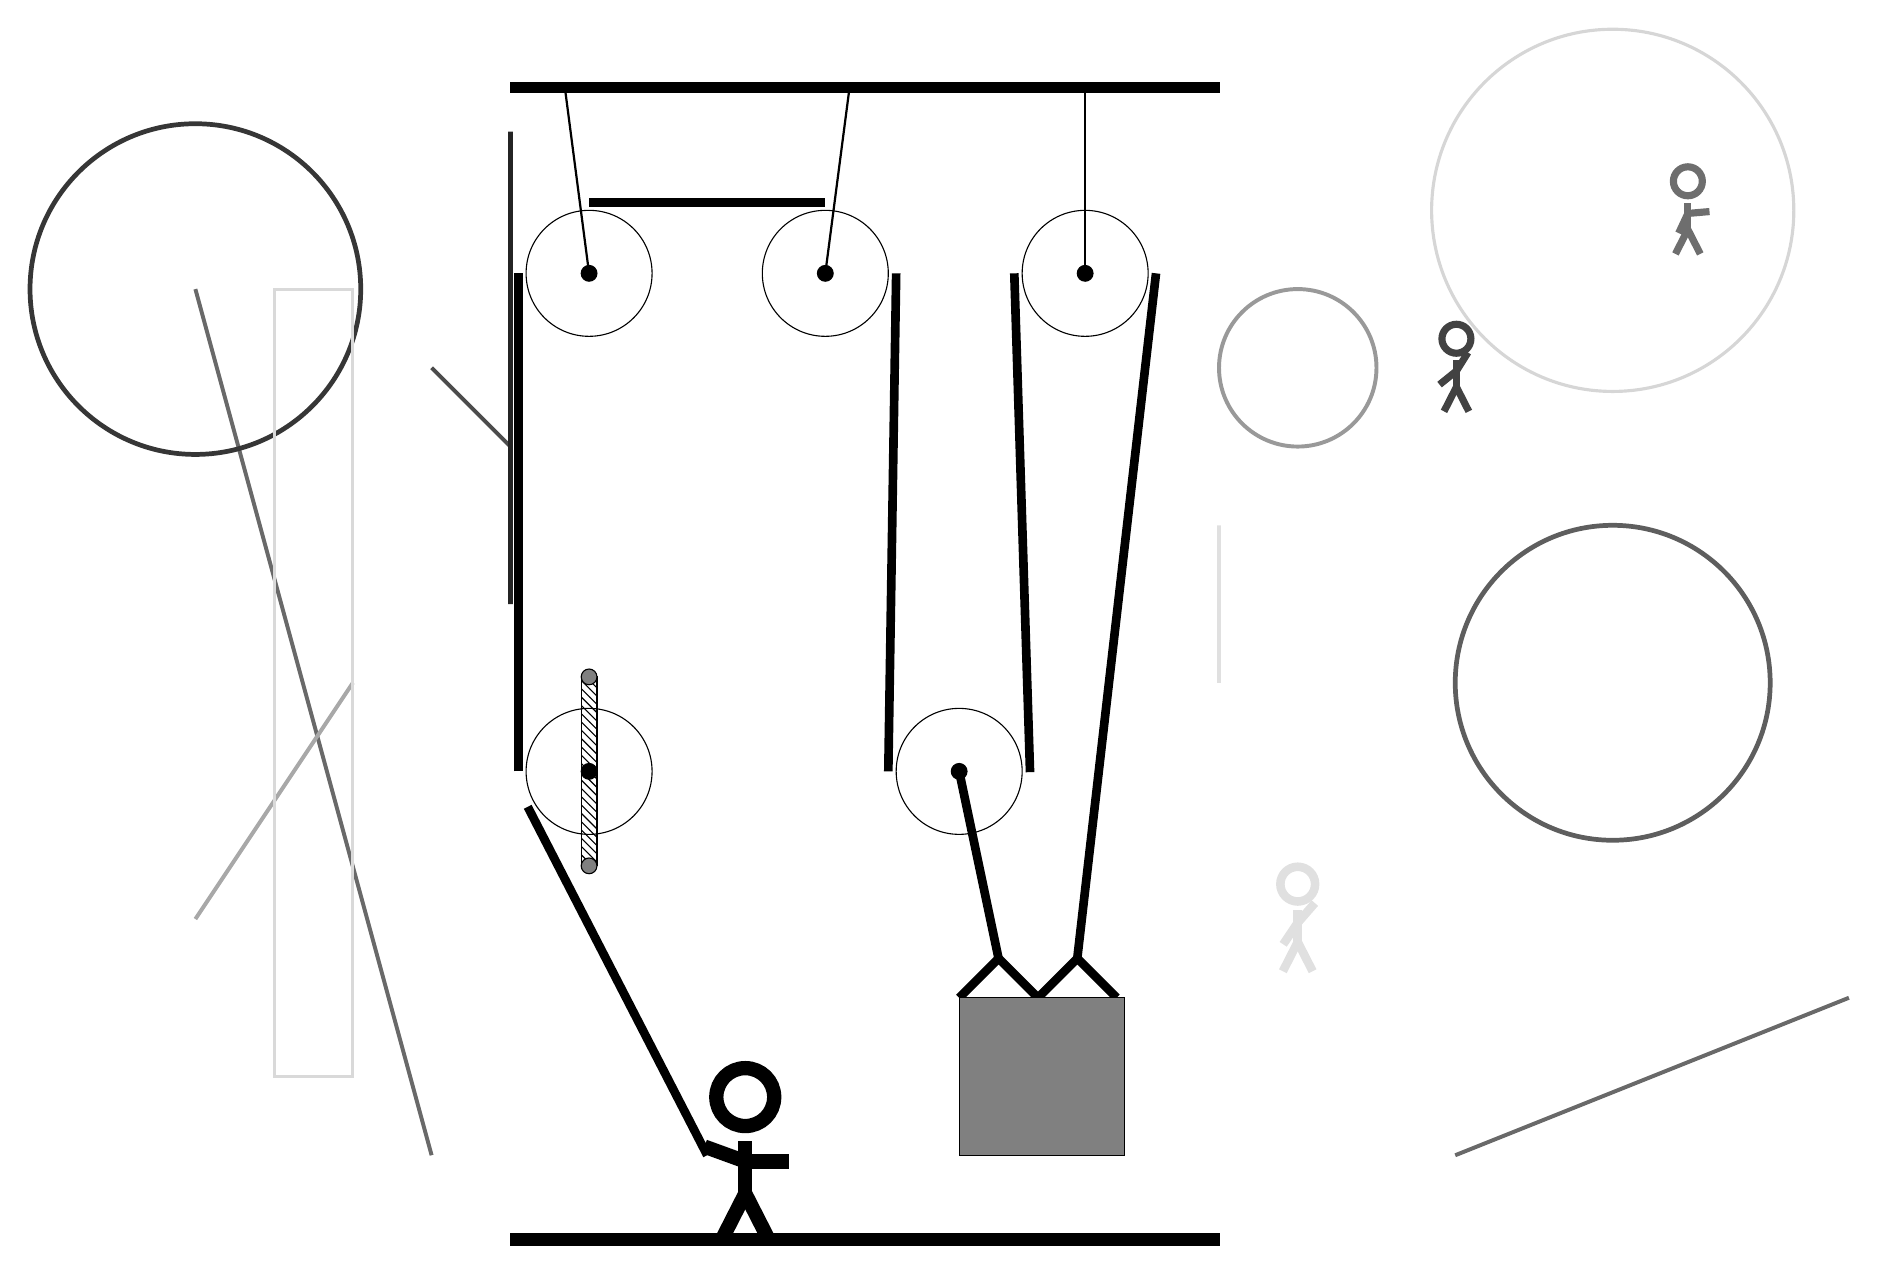
\begin{tikzpicture}
			%%%%% START %%%%%
			
			\draw[fill=black] (-3, 11.5) rectangle (6, 11.625);
			
			\draw (1, 9.2) circle (0.8);
			\draw[fill=black] (1, 9.2) circle (0.1);
			\draw[thick] (1, 9.2) -- (1.3, 11.5);
			
			\draw (4.3, 9.2) circle (0.8);
			\draw[fill=black] (4.3, 9.2) circle (0.1);
			\draw[thick] (4.3, 9.2) -- (4.3, 11.5);
			
			\draw[line width=0.5mm, color=black!59](9, -2) -- (14, 0);
			
			\node[line width=0.7mm, color=black!74] at (9, 8) {\Strichmaxerl[5][39][58]};
			\node[line width=0.2mm, color=black!57] at (12, 10) {\Strichmaxerl[5][65][5]};
			\draw[line width=0.5mm, color=black!70](-3, 7) -- (-4, 8);
			
			\draw[line width=0.6mm, color=black!86] (-3, 5) rectangle (-3, 11);
			\draw[line width=0.5mm, color=black!59](-4, -2) -- (-7, 9);
			
			\draw [line width=0.6mm, color=black!79](-7, 9) circle (2.1);
			\draw [line width=0.6mm, color=black!63](11, 4) circle (2.0);
			\draw [line width=0.4mm, color=black!16](11, 10) circle (2.3);
			\draw [line width=0.5mm, color=black!40](7, 8) circle (1.0);
			\draw[line width=0.5mm, color=black!34](-5, 4) -- (-7, 1);
			
			\draw[line width=0.4mm, color=black!12] (6, 4) rectangle (6, 6);
			\draw[line width=0.4mm, color=black!15] (-5, 9) rectangle (-6, -1);
			
			\node[line width=0.4mm, color=black!12] at (7, 1) {\Strichmaxerl[6][56][49]};
			
			\draw (2.7, 2.875) circle (0.8);
			\draw[fill=black] (2.7, 2.875) circle (0.1);
			
			\draw[line width=1.1mm]  (2.7, 0.0) -- (3.2, 0.5) -- (3.7, 0.0) -- (4.2, 0.5) -- (4.7, 0.0);
			\draw[fill=black!50] (2.7, 0.0) rectangle (4.8, -2.0);
			
			\draw (-2, 9.2) circle (0.8);
			\draw[fill=black] (-2, 9.2) circle (0.1);
			\draw[thick] (-2, 9.2) -- (-2.3, 11.5);
			
			\draw (-2, 2.875) circle (0.8);
			\draw[fill=black] (-2, 2.875) circle (0.1);
			\draw[pattern=north west lines, pattern color=black] (-2.1, 4.075) rectangle (-1.9, 1.675);
			\draw[fill=black!50] (-2, 4.075) circle (0.1);
			\draw[fill=black!50] (-2, 1.675) circle (0.1);
			
			\draw[line width=1.1mm](-0.5, -2) -- (-2.7794, 2.425);
			\centerarc[line width=1.1mm](-2, 2.875)(180:210:0.9);
			\draw[line width=1.1mm](-2.9, 2.875) -- (-2.9, 9.2);
			\centerarc[line width=1.1mm](-2, 9.2)(90:180:0.9);
			
			\draw[line width=1.1mm](-2, 10.1) -- (1, 10.1);
			\centerarc[line width=1.1mm](1, 9.2)(0:90:0.9);
			\draw[line width=1.1mm](1.9, 9.2) -- (1.8, 2.875);
			\centerarc[line width=1.1mm](2.7, 2.875)(180:370:0.9);
			\draw[line width=1.1mm] (3.6, 2.865) -- (3.4, 9.2);
			\centerarc[line width=1.1mm](4.3, 9.2)(0:180:0.9);
			\draw[line width=1.1mm](4.2, 0.5) -- (5.2, 9.2);
			\draw[line width=1.1mm] (3.2, 0.5) -- (2.7, 2.875);
			
			\node at (0, -2) {\Strichmaxerl[10][-20][0]};
			
			\draw[fill=black] (-3, -3) rectangle (6, -3.15);
			
			%%%%% END %%%%%
		\end{tikzpicture}
	\end{figure}	
\end{document}